%%%%%%%%%%%%%%%%%%%%%%%%%%%%%%%%%%%%%%%%%%%%%%%%%%%%%%%%%%%%%%%%%%%%%%%%%%%%%%%%
%2345678901234567890123456789012345678901234567890123456789012345678901234567890
%        1         2         3         4         5         6         7         8

\documentclass[letterpaper, 10 pt, conference]{ieeeconf}  % Comment this line out if you need a4paper

%\documentclass[a4paper, 10pt, conference]{ieeeconf}      % Use this line for a4 paper

\IEEEoverridecommandlockouts                              % This command is only needed if 
                                                          % you want to use the \thanks command

\overrideIEEEmargins                                      % Needed to meet printer requirements.

%In case you encounter the following error:
%Error 1010 The PDF file may be corrupt (unable to open PDF file) OR
%Error 1000 An error occurred while parsing a contents stream. Unable to analyze the PDF file.
%This is a known problem with pdfLaTeX conversion filter. The file cannot be opened with acrobat reader
%Please use one of the alternatives below to circumvent this error by uncommenting one or the other
%\pdfobjcompresslevel=0
%\pdfminorversion=4

% See the \addtolength command later in the file to balance the column lengths
% on the last page of the document

% The following packages can be found on http:\\www.ctan.org
\usepackage{graphicx} % for pdf, bitmapped graphics files
%\usepackage{epsfig} % for postscript graphics files
%\usepackage{mathptmx} % assumes new font selection scheme installed
%\usepackage{times} % assumes new font selection scheme installed
\usepackage{amsmath} % assumes amsmath package installed
%\usepackage{amssymb}  % assumes amsmath package installed

\title{\LARGE \bf
Hands-Free: a robot augmented reality teleoperation system
}

%\author{\authorblockN{Cristina Nuzzi\authorrefmark{1}, Stefano Ghidini\authorrefmark{2}, Roberto Pagani\authorrefmark{1}, Simone Pasinetti\authorrefmark{1} and Giovanna Sansoni\authorrefmark{1}}
%\authorblockA{\authorrefmark{1} University of Brescia, Department of Mechanical and Industrial Engineering, Via Branze 38, 25123 Brescia, Italy\\
%e-mail: c.nuzzi@unibs.it, r.pagani001@unibs.it, simone.pasinetti@unibs.it, giovanna.sansoni@unibs.it}
%\authorblockA{\authorrefmark{2} STIIMA-CNR, Via Alfonso Corti 12, 20133 Milan, Italy\\
%e-mail: stefano.ghidini@stiima.cnr.it}
%}

\author{Cristina Nuzzi$^{*}$, Stefano Ghidini, Roberto Pagani, Simone Pasinetti and Giovanna Sansoni % <-this % stops a space
\thanks{This work was not supported by any organization.}% <-this % stops a space
\thanks{Cristina Nuzzi, Roberto Pagani, Simone Pasinetti and Giovanna Sansoni are members of the Department of Mechanical and Industrial Engineering at University of Brescia, Via Branze 38, 25123 Brescia, Italy.}
\thanks{Stefano Ghidini is a member of the STIIMA-CNR, Via Alfonso Corti 12, 20133 Milan, Italy. He is also a member of the Department of Mechanical and Industrial Engineering at University of Brescia, Via Branze 38, 25123 Brescia, Italy.}
\thanks{$^{*}$ Corresponding author, e-mail: {\tt\small c.nuzzi@unibs.it}}%
}

\begin{document}

\maketitle
\thispagestyle{empty}
\pagestyle{empty}

%%%%%%%%%%%%%%%%%%%%%%%%%%%%%%%%%%%%%%%%%%%%%%%%%%%%%%%%%%%%%%%%%%%%%%%%%%%%%%%%
\begin{abstract}

This electronic document is a live template. The various components of your paper [title, text, heads, etc.] are already defined on the style sheet, as illustrated by the portions given in this document.

\end{abstract}


%%%%%%%%%%%%%%%%%%%%%%%%%%%%%%%%%%%%%%%%%%%%%%%%%%%%%%%%%%%%%%%%%%%%%%%%%%%%%%%%
\section{INTRODUCTION}
Despite advances in robotic perception are increasing autonomous capabilities, the human intelligence is still considered a necessity in unstructured or not predictable environments. Typical scenarios concern the detection of random shape objects, manipulation, or custom robot motion. In such context, human and robots must achieve mutual human-robot interaction (HRI) \cite{Yanco2002}.

HRI can be both physical (pHRI) or not, depending on the assigned task. For example, when the robot is constrained in a dangerous environment or must handle hazardous materials, pHRI is not recommended. In this cases, robot teleoperation may be necessary. A teloperation system concerns with the exploration and exploitation of spaces which do not allow user presence, thus, the operator acts by remotely move the robot \cite{VERTUTJean}. A plenty of human-machine interfaces for teleoperation have been developed considering a mechanical interface, this includes exoskeleton \cite{Rebelo2014} or gloves \cite{Lv2006}. Such systems are particularly helpful to achieve bilateral teleoperation \cite{Hokayem2006}, where they can transmit or reflect back to the user reaction forces from the task being performed. In this case, a high perception with complete haptic feedback \cite{Glover2009} is achieved. Other controllers includes mouse, switchbox, keyboard, touch-screen and joystick, which is usually a better control device than others because the operators can identify better with the task \cite{Boboc2012}. Among the systems where bilateral teleoperation is not required, a teleoperation system is defined by mean of electromyography (EMG) signals of the muscular activity \cite{Vogel2011, Hassan2019}. However, as reminded recently in \cite{Roveda2018a}, EMG could be affected by difficulties in processing EMG signals for amplitude and spectral analysis, reducing their efficiency for many applications. Moreover, all this interfaces still act by contact, hindering the movement of the operator or cause him to act through unnatural movements.

On the other side, if bilater interaction is not required, a vision-based interface is preferable. A vision-based interface does not require physical contact with external devices such as cables, connectors and objects outside of the user working area. This grants a more natural and intuitive interaction, which is reflected on the task performance: as shown in \cite{Kofman2005}, the accuracy of object gripping tasks is improved by mean of a contactless vision-based robot teleoperation method, while in \cite{Livatino2009} a stereo vision system improved the performance of a mobile robot teleoperation application.

Furthermore, if a vision-interface is integrated with virtual and augmented reality techniques, it translates in a greater level of immersion for the user. Such techniques are used to enhance the feedback information; in fact, the operator feels like being physically present in the remote environment, enhancing the immersion level. The notion of immersion is one of the most important reasons for using virtual and augmented reality \cite{Boboc2012}. An augmented reality system for teleoperation based on the Leap Motion (LM) controller is presented in \cite{Peppoloni2015}. For its application domain, the LM controller is considered an accurate sensor \cite{Hedayati2018}, however it is limited to a relatively small measuring distance if compared with other sensors. In this sense, the LM controller introduces spatial constraints that clash with the previously stated concept of the high level user immersion.

For these reasons, we present a novel robot augmented reality teleoperation system that exploits RGB cameras, which provide greater measuring distance if compared with the LM controller. A ROS-based framework has been developed to provide hand tracking and hand-gesture recognition features, exploiting the OpenPose software \cite{simon2017hand, cao2018openpose} based on the Deep Learning framework Caffe \cite{jia2014caffe}.
This, in combination with the ease of availability of an RGB camera, lead the framework to be strongly open-source oriented and highly replicable on all the ROS-based platform. The proposed system includes: neural network for hand$-$gesture recognition (Section \ref{sec:HG_recon}), a rigorous procedure for robot workspace calibration and a mapping policy between the coordinate system of the user and the robot (Section \ref{sec:HG_recon}). 
Different experiments were performed on a \textit{Sawyer (Rethink Robotics)} industrial collaborative robot to evaluate repeatability and accuracy of the proposed system. Section \ref{sec:experiments} reports the results.

\section{Workspace Calibration and Mapping} \label{sec:calib}
Our set-up is composed of two workspaces: the \textit{user workspace} and the \textit{robot workspace}. Cartesian points in the user workspace that can be reached by the user hand and are correctly viewed by the camera correspond to precise robot end-effector Cartesian points in the robot workspace. To obtain the mapping between the hand positions and the robot end-effector positions, it is necessary to perform a set of calibration procedures described in detail in the following sections.

\subsection{User Workspace Calibration}
In the user workspace an RGB camera is used to recognize the hand skeleton in real-time. Therefore, it is necessary to properly calibrate the camera with respect to the user-defined reference system. This procedure is called \textit{camera calibration}, and can be easily realized following standard procedures, such as the one detailed in \cite{MatlabCameraCalib}.
To correctly map a point $S = (U, V)$ in the image to its corresponding real world coordinate $P = (X, Y, Z)$ it is necessary to apply the following formula:
\begin{equation}
s 
  \begin{bmatrix}
    U \\
    V \\
    1
  \end{bmatrix}
 =
K
  \begin{bmatrix}
    R | t
  \end{bmatrix}
  \begin{bmatrix}
    X \\
    Y \\
    Z \\
    1
  \end{bmatrix}
\label{eq1}
\end{equation}

In the formula, the scalar \textbf{s} is the scale factor of the image, matrix \textbf{K} is the camera matrix containing the intrinsic parameters of the camera such as focal length and optical center, and the \textbf{[R$|$t]} matrix is the rigid transformation matrix containing the exstrinsic parameters rotation \textbf{R} ($3$x$3$ matrix) and translation \textbf{t} ($3$x$1$ matrix) of the camera reference system $C$ with respect to the calibration master reference system $H$.
To obtain matrix \textbf{K} it is necessary to perform a calibration procedure. A well-performed calibration procedure allows to obtain a satisfactory estimation of the camera parameters. To correctly map image points to the corresponding real world coordinates, the rigid transformation matrix must be estimated with respect to the user-defined reference system of the calibration master. Thus, if reference system $H$ changes or the camera $C$ moves, it is necessary to estimate again the correct rigid transformation matrix. % this procedure has been automatized by our software.

Images acquired by the camera are processed and the hand skeleton joints coordinates are calculated. By using the abovementioned formula, for each frame it is possible to obtain the real world coordinates of the hand skeleton joints in real time (Fig. \ref{fig:w1}).

\begin{figure} [h!]
  \centering
  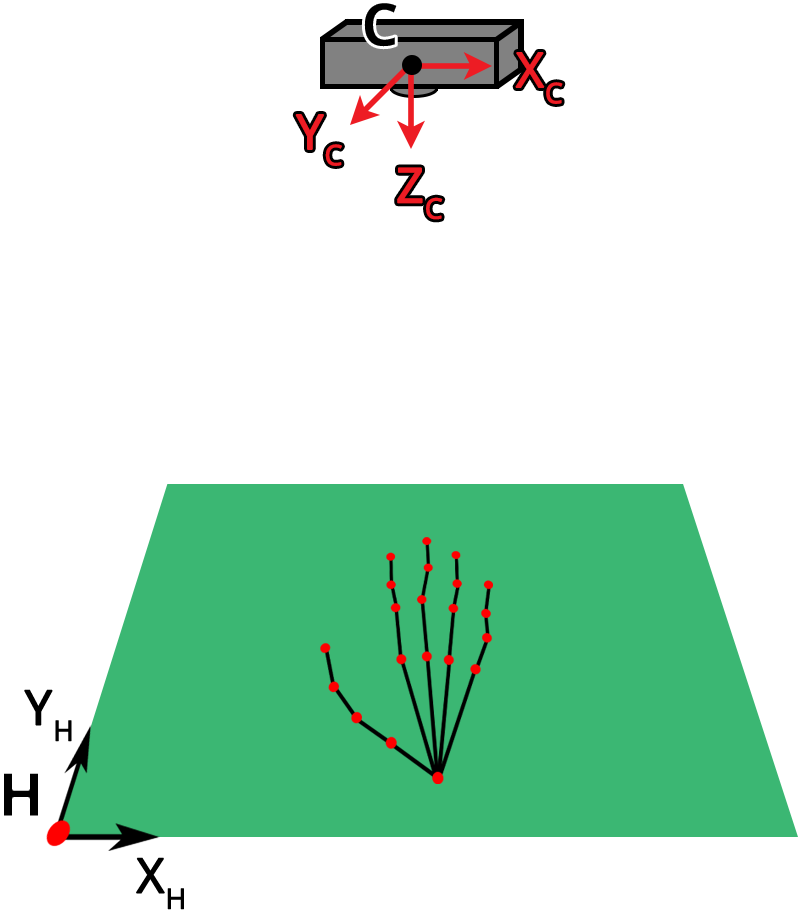
\includegraphics[width=0.5\columnwidth]{figures/w1.png}
  \caption{Scheme of the user workspace, where the camera reference system $C$ and the user-defined reference system $H$ are calibrated to find the correspondence between image points and real world coordinates.}
  \label{fig:w1}
\end{figure}

%% img del set up di calibrazione matlab
% risultati di calibrazione? Img della mano con skeleton?

\subsection{Robot Workspace Calibration}
The robot workspace refers to the space in which the robot moves (purple square of Fig. \ref{fig:w2}) with respect to the user workspace (green square of Fig. \ref{fig:w1}). In this case, the user hand real-world position in reference system $H$ is mapped to the new reference system $W$. The mapping between reference system $H$ and reference system $W$ is obtained easily if the two workspaces have the same dimension (matrix \textbf{[R$|$t]} is the identity matrix) or if one workspace is a scaled version of the other one (matrix \textbf{[R$|$t]} is the identity matrix multiplied by the scale factor). %verificare

\begin{figure} [h!]
  \centering
  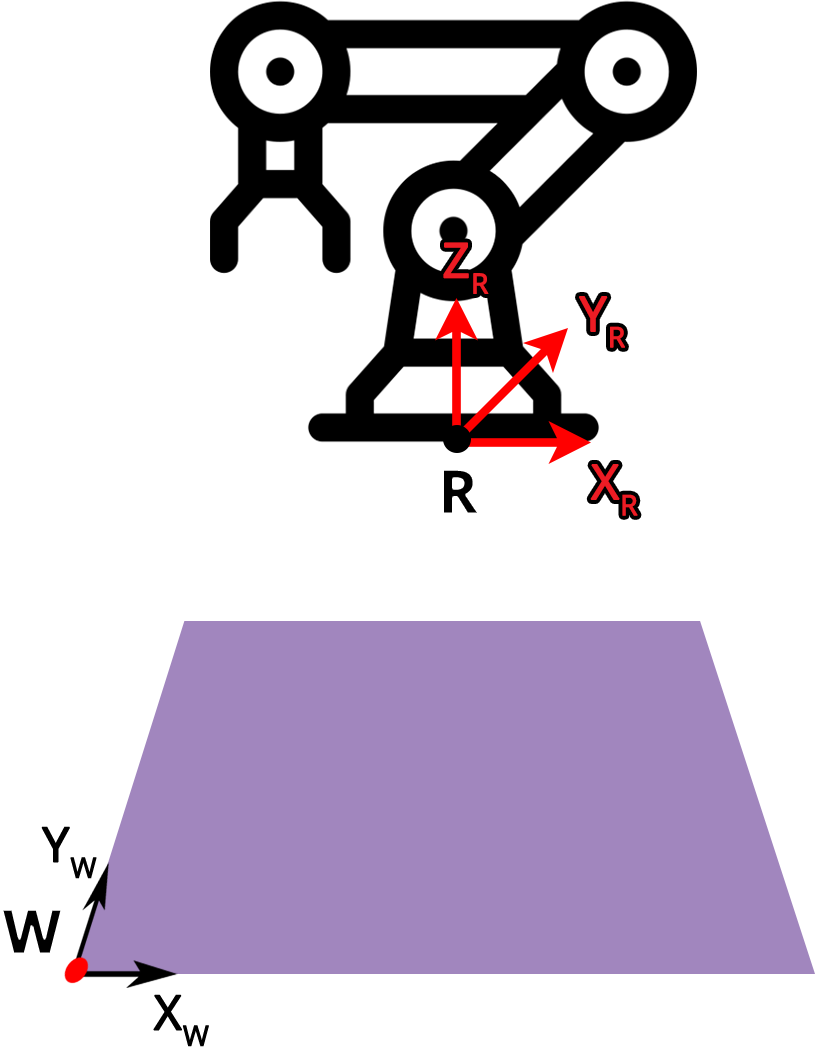
\includegraphics[width=0.5\columnwidth]{figures/w2.png}
  \caption{Scheme of the robot workspace, where the second user-defined reference system $W$ and the robot reference system $R$ are calibrated to find the correspondence between the workspace positions and the end-effector joint coordinates.}
  \label{fig:w2}
\end{figure}

To correctly move the robot in a cartesian position of reference system $W$, it is necessary to perform a calibration between reference system $W$ and the robot reference system $R$. This procedure has been carried out experimentally by moving the robot (using its manual guidance mode) in a set of $13$ Cartesian positions of reference system $W$ (Fig. xx). % check fig master
The robot correct positioning on top of each calibration position has been assured by using a 3D-printed centering tool (Fig. xx): the tool must be centered manually on each calibration marker and secured in place, then the robot end effector can be moved on it and carefully positioned inside the purposely made circular cavity of the tool. When the positioning is complete, the robot coordinates (both in the Cartesian space and in the Joints space) corresponding to that particular marker (of which the positioning is known with respect to reference system $W$) can be extracted using ROS or the robot proprietary software.

When a satisfactory number of calibration positions (in our case, $13$) has been acquired, it is possible to estimate the rigid transformation matrix between workspaces $W$ and $R$, following the formula: %% formula simo

\section{Hand-Gesture Recognition}\label{sec:HG_recon}
%Che rete uso, come ho impostato i gesti, lo scheletro con openpose citato, funzione per ricavare il gesto basata sull'assenza del finger, invariante dall'orientamento e dallo zoom. Immagini di esempio.

The proposed teleoperation method is based on the recognition of the user hands skeleton.

Each frame acquired by the RGB camera (in our set-up, a Kinect v2 camera) is processed by the software, which leverages the OpenPose hand skeleton recognition network to predict the hand skeleton, following the details of \cite{simon2017hand}.
The gesture recognition procedure is based on the position of the reference keypoint (red keypoint $0$ in Fig. \ref{fig:keypoints}) and on the position of the four knuckles keypoints (blue keypoints $5, 9, 13, 17$ in Fig. \ref{fig:keypoints}). According to the knuckles and the thumb $(x, y)$ keypoints positions (from keypoint $1$ to $4$), the hand orientation can be hypotized as upright, left oriented, right oriented, or upside down. This allows the software to recognize the gestures regardless of the hand orientation. %% prendere img di una mano e fare gli esempi di posizionamento, cambiare i colori dei marker

To recognize if a certain finger is opened or closed, we consider the Euclidean distance between the reference keypoint $0$ and the last keypoint of each finger (pink keypoints $8, 12, 16, 20$ in Fig. \ref{fig:keypoints}). If the last keypoint of a finger is not recognized by the network, we consider the corresponding Euclidean distance equal to $0$. 
Using this logic, we defined two gestures used to carry out basic teleoperation tasks: the \textbf{open hand} gesture, where all the fingers are detected as opened, and the \textbf{index} gesture, where the index finger is detected as open and with a corresponding Euclidean distance much greater than the Euclidean distances of the other fingers. This requirement has been proved useful to reduce the recognition error of the index gesture due to a wrong prediction of the fingers keypoints.

\begin{figure} [h!]
  \centering
  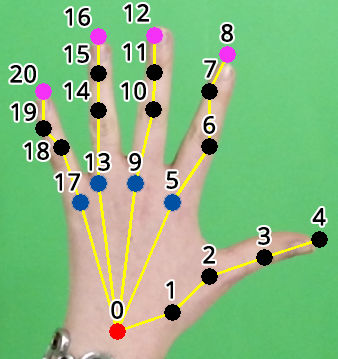
\includegraphics[width=0.7\columnwidth]{figures/hand.png}
  \caption{Example of an open hand gesture correctly recognized skeleton. The red keypoint is the reference keypoint, the blue keypoints are the knuckles keypoints and the pink keypoints are the fingertips keypoints.}
  \label{fig:keypoints}
\end{figure}

Considering the calibration procedure detailed in Section \ref{sec:calib}, a certain position $P_H$ of user workspace H corresponds to a certain robot end-effector position $P_W$ in workspace W. Hence, to move the robot end-effector in position $P_W$  using the software, users must: %img
\begin{enumerate}
\item place their hand in position $P_H$ (corresponding to position $P_W$), using the real-time visualization of the software as guidance (Fig. xx a);
\item perform the open hand gesture to allow the coordinate extraction (Fig. xx b);
\item perform the index gesture, carefully pointing the index finger to position $P_H$ (Fig. xx c).
\end{enumerate}

It is worth noting that, since the hand skeleton is obtained by a neural network which estimates the joints coordinates frame per frame, their position in consectuive frames may vary. Therefore, our software extracts $N$ different $P_H$ coordinates from $N$ consecutive index gestures recognized in consecutive frames. The average coordinates are extracted to reduce positioning errors introduced by the hand skeleton recognition network. The higher the value of $N$, the higher the error reduction, at the cost of a higher delay before the final $P_H$ coordinates are extracted. In our set-up, we set $N = 7$.
After a position $P_H$ is obtained, the corresponding robot position $P_R$ is calculated and the robot is moved there using ROS.
To perform a new robot movement, the procedure in Fig. xx must be repeated from the start.

\section{EXPERIMENTAL EVALUATION}\label{sec:experiments}
A reliable teleoperation system is obtained if the robot correctly moves to the desired position with a low positioning error. In the case of the proposed set-up, the positioning error is obtained as a sum of different positioning errors, obtained as follows:
\begin{enumerate}
\item thanks to the camera calibration procedure, a certain index finger position $P_C$ [px] in the acquired image frame corresponds to a certain Cartesian point $P_H$ [mm] in workspace $H$. Since the camera calibration procedure introduces an estimation error $E_1$, we obtain $P_H = P_C + E_1$;
\item our software extracts $N$ consecutive finger positions estimated by OpenPose neural network and calculates the average of them. The resulting point is $P_O = \frac{\sum_{n=1}^{N}(P_{Hn} + E_{2n})}{N}$, where $E_2$ is the error between the real position of the index finger in the image and the index keypoint estimation made by OpenPose;
\item the extracted index finger position $P_O$ corresponds to a certain Cartesian point in workspace $W$. According to the mapping between workspace $H$ and $W$, we obtain $P_W = P_O + E_3$, where $E_3$ is the positioning error caused by this mapping;
\item the robot end-effector will move in cartesian point $P_R$, obtained considering the rigid transformation between workspaces $W$ and $R$. This transformation introduces the positioning error $E_4$, thus we obtain $P_R = P_W + E_4$.
\end{enumerate}

Hence, we obtain the final end-effector position $P_R$ as: 
\begin{equation}
P_R =\frac{\sum_{n=1}^{N}(P_{Cn} +  E_{1n} +  E_{2n})}{N} + E_3 + E_4
\end{equation}
Considering this formula, and that in our set-up $E_3$ can be assumed equal to zero (because we kept workspace $H$ and workspace $W$ dimensions except for the scaling factor), we designed two experiments to assess if the positioning error obtained depends (i) on the camera calibration ($E_1$), (ii) on the estimation of the hand skeleton ($E_2$), or (iii) on the robot calibration ($E_4$).

\subsection{Evaluation of the skeleton estimation error}
The positioning error due to the estimation of the hand skeleton joints made by OpenPose neural network has been evaluated considering the theoretical position of the index in the image $T$ and the index joint position in the image $A$ calculated by the software (Fig. xx).
%% risultati e commento

\subsection{Evaluation of the robot positioning error}
In our set-up, reference system $H$ is placed horizontally with the camera mounted still at a $1 m$ distance (Fig. xx). Reference system $W$, however, has been placed vertically on a glass pane (Fig. xx).
To reliably assess the positioning of the robot end-effector, a red laser has been mounted on the end effector (laser name bla bla) (Fig. xx). When the robot is moved to a certain theoretical position $T$, the laser will point to its actual positioning $A$. To correctly visualize and measure the robot workspace and the laser positioning, an RGB camera (camera serial name) has been mounted behind the glass pane.
A measuring software has been developed using LabVIEW to measure the distance between the theoretical position $T$ (calculated as the barycenter of the black dot of the experimental master as in Fig. xx) and the actual positioning $A$ (red dot in the image as in Fig. xx).

We moved the robot using the proposed system in $xx$ theoretical positions. To do that, we used the Cartesian positions corresponding to the circular markers barycenters (theoretical positions) to move the robot using ROS. Hence, this procedure avoids considering the hand skeleton estimation errors.
%% risultati e commento



\section{Figures and Tables}

\begin{table}[h]
\caption{An Example of a Table}
\label{table_example}
\begin{center}
\begin{tabular}{|c||c|}
\hline
One & Two\\
\hline
Three & Four\\
\hline
\end{tabular}
\end{center}
\end{table}

\section{CONCLUSIONS}

Conclusioni sul progetto/esperimenti ottenuti.
Problematiche incontrate e come sono state risolte.
Future developments.

\addtolength{\textheight}{-12cm}   % This command serves to balance the column lengths
                                  % on the last page of the document manually. It shortens
                                  % the textheight of the last page by a suitable amount.
                                  % This command does not take effect until the next page
                                  % so it should come on the page before the last. Make
                                  % sure that you do not shorten the textheight too much.
%Hands-free
%%%%%%%%%%%%%%%%%%%%%%%%%%%%%%%%%%%%%%%%%%%%%%%%%%%%%%%%%%%%%%%%%%%%%%%%%%%%%%%%%
%
%\bibliographystyle{ieeetr}
%\bibliography{/home/abel/Documenti/Mendeley_References/LuGre}


\bibliographystyle{ieeetr}
\bibliography{bibliography}


\end{document}
